\documentclass[12pt]{article}
%\usepackage{times}
\usepackage{cite}
\usepackage{graphicx}
%this is a comment
\title{Software Requirements and Planning: CommunityConnect}
\author{Kamron Ebrahimi \& Samuel Wilson \& Leif Tsang \& Thomas Korsness \& Quinton Osborn \\ ebrahimk, wilsosam, tsangl, korsnest, osbornq}
\date{\today}

\begin{figure}
	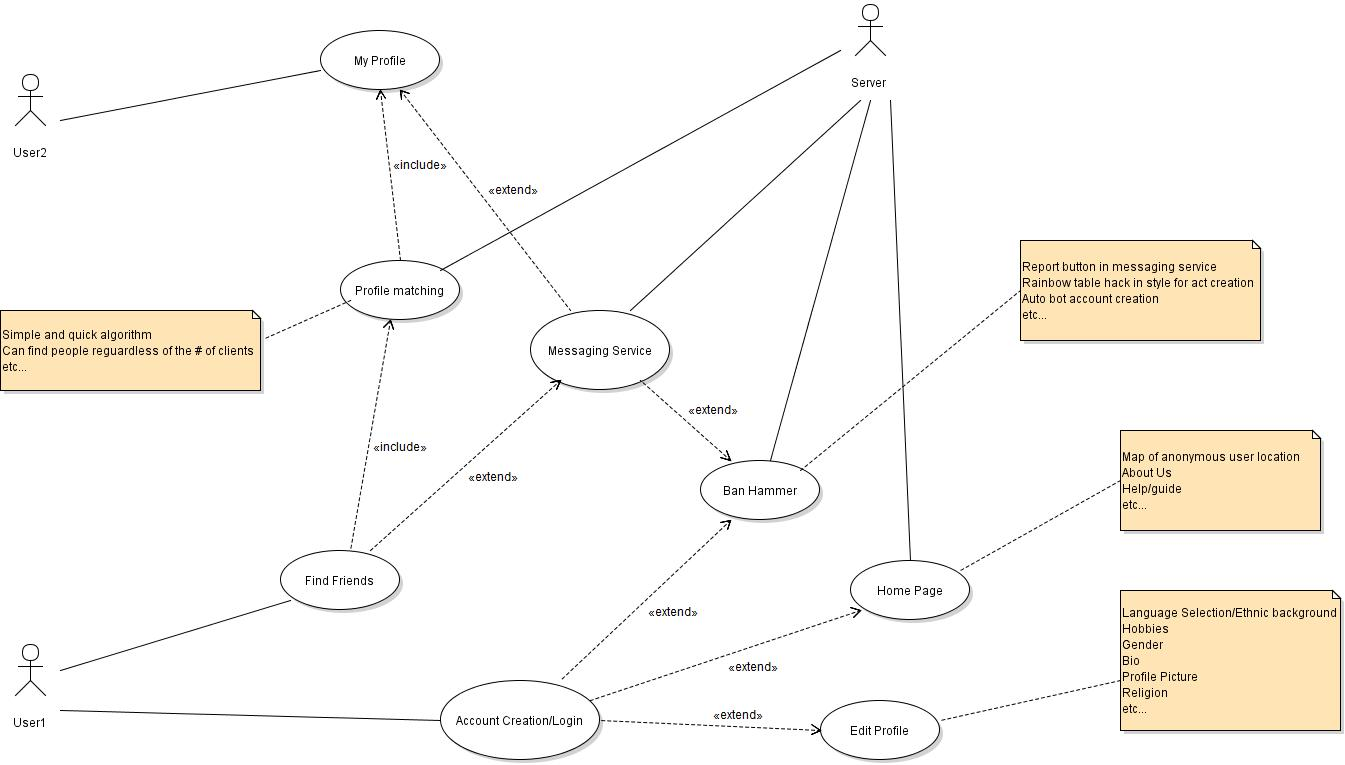
\includegraphics[width=\linewidth]{useCaseDiagram.jpg}
	\caption{Use Case Diagram}
	\label{fig:UseCase}
\end{figure}

\begin{figure}
	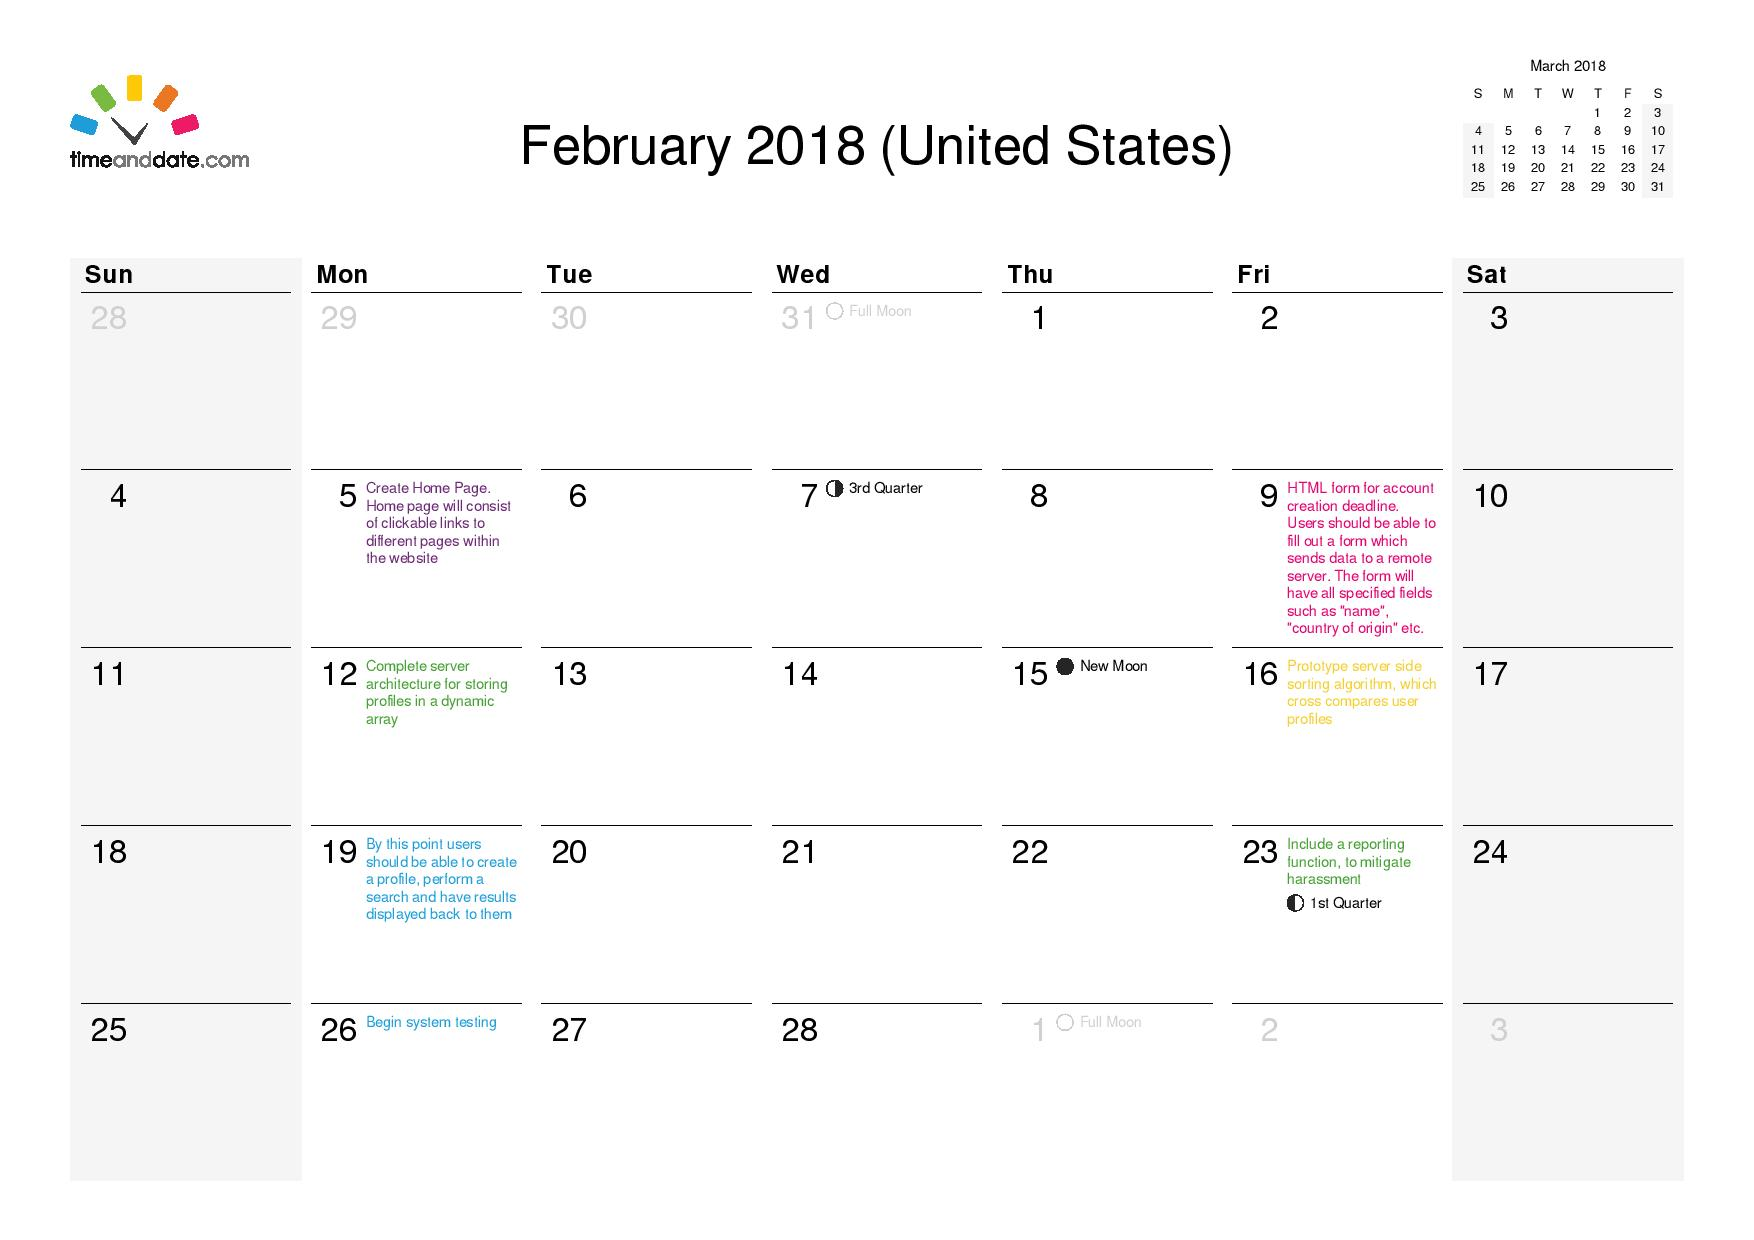
\includegraphics[width=\linewidth]{february.jpg}
	\caption{February Timeline}
	\label{fig:february}
\end{figure}

\begin{figure}
	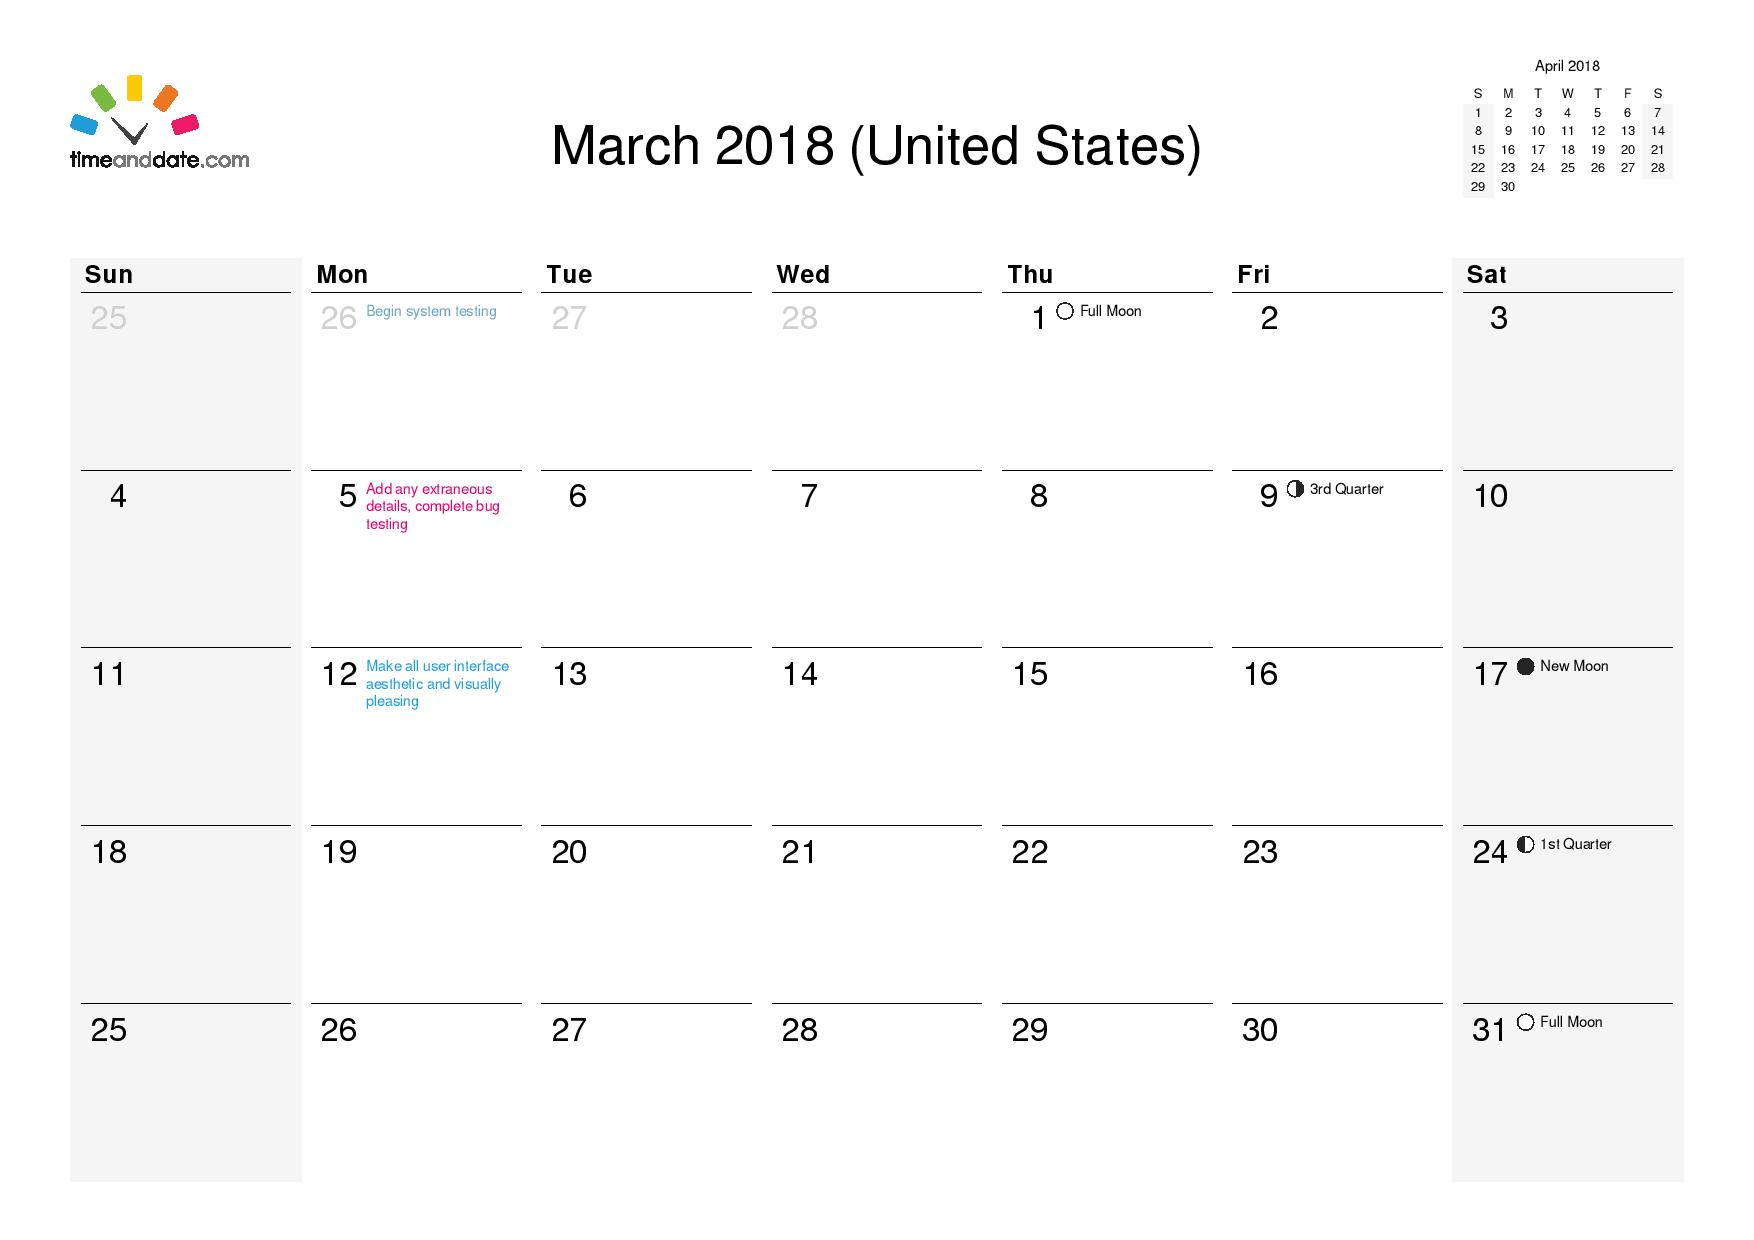
\includegraphics[width=\linewidth]{march.jpg}
	\caption{March Timeline}
	\label{fig:march}
\end{figure}

\begin{document}

\maketitle

\tableofcontents

\section{\bf Project Description}
	\subsection{\bf Approach}
		\paragraph{\normalfont \indent CommunityConnect is a web-based application used to help individuals from diverse ethnic backgrounds build a social support network. CommunityConnect achieves this through a simple matching algorithm. Users will create an account, in which they submit information such as their ethnic background, religion, language, a brief biography, contact information and location, and their accounts information will be cross compared with other user accounts, looking for other individuals with the same cultural background within some given mile radius.
		}
		\paragraph{\normal \indent CommunityConnect targets displaced individuals or immigrants living in the United States. A host of scientific inquiries have been made into the effects of support networks among displaced individuals and immigrants. The 2014 study, \textit{Social isolation and perceived barriers to establishing social networks among Latina immigrants} ~\cite{Cite1}, found that “perceived social isolation and lack of social support negatively impact health” and  that many immigrants unaccustomed to US culture report “feeling lonely, isolated, closed-in, and less free in the US due to family separation and various obstacles to develop and maintain relationships.” This is not the only study to yield such results in fact there is a specific term for this phenomena coined “cultural isolationism.” The 2010 study \textit{Social support and health: immigrants and refugees perspectives} ~\cite{Cite2}, investigated the effects of social support on the utilization of public services among refugees and immigrants and found that there exist a positive correlation between the two. This study further reinforces the need for some web based application like CommunityConnect.
		}
	\subsection{\bf Innovation}
		\paragraph{\normalfont \indent There are many humanitarian web-based applications which serve to connect immigrants or refugees with local resources or with lost family members and friends. Similarly the web application Meetup allows user to join groups based off of their ethnicity, and designated, user-organized events for large groups of people in metropolitan areas. CommunityConnect would personalize the user experience even more and potentially serve immigrants/refugees who move to more rural locations by finding individuals who share the users cultural background who are physically close by. If a person who lived in a rural community used Meetup they would potentially have to travel sometime to gathering location and then be exposed to a large gathering of people who may already be acquainted with one another. CommunityConnect would connect people on an individual and geographical basis so users can build close knit relations even in rural areas.
		}
	\subsection{\bf Tools}
		\paragraph{\normalfont \indent CommunityConnect would require a variety of different programming languages for both client and server side interactions. On the client side, languages such as HTML, CSS, and Javascript would be used to create an aesthetic webpage interface for the user. PHP will be used to write the matching algorithm on the server side of the process. HTML, CSS, and JavaScript are standard client-side web development languages and all members of the CommunityConnect group are familiar with these programming languages, thus no time will be wasted getting members up to speed. PHP will be the server side scripting language used to develop CommunityConnect. As a team CommunityConnect needs to get up to speed on server side scripting, however we are selecting PHP as our the primary server side scripting language because some members of the team have fundamental skills with the language.
		}
	\subsection{\bf Requirements}
		\subsection{\bf Functional}
			\begin{enumerate}
				\item The user will be able to create a profile containing their contact information containing but not limited to:
					\begin{enumerate}
						\item Contact Information
						\item Location
						\item Ethnic Background
						\item Country of Origin
						\item Religion
					\end{enumerate}
				\item The user will be able to perform a search for others within a certain mile radius of their location
				\item	Searches will return the contact information of other uses with identical ethnic backgrounds
				\item
			\end{enumerate}
		\subsection{\bf Non-Functional}
			\item CommunityConnect will securely maintain user profile information
			\item CommunityConnect will return search results within 1 minute of processing a request
			\item Profiles of individuals are only public to the user if they match with that individual
	\subsection{\bf Documentation and Features}
		\paragraph{\normalfont \indent CommunityConnect will have a home webpage on which will be hosted a brief biography about the developers, a setting option allowing users to swap between the language in which the page is displayed and a brief guide on how CommunityConnect works. The guide will be the users main resource for questions regarding the use of the application.
		}
		\paragraph{\normalfont The four major features of CommunityConnect which make it so useful are as follows:}
		\begin{itemize}
			\item Personalized profile creation containing contact information, biography, cultural background
			\item Intricate profile matching algorithm which generates matches based off user location and ethnic background
			\item A simple reporting system for protecting users from harassment, and a system for banning/holding and an account
			\item A homepage with a user guide and statistics/graphic on the applications traffic in different locations
		\end{itemize}

\section{\bf Use Cases}
  \subsection{\bf Diagram}

		Figure \ref{fig:UseCase} Use Case diagram

	\subsection{\bf Use Case 1}
		\subsubsection{Use Case Name}
			\paragraph{\normalfont Friend Matching
  		}
		\subsubsection{Goal Level}
			\paragraph{\normalfont Create an algorithm which allows people to find others near them with the same cultural background.
	  	}
		\subsubsection{Actor}
			\paragraph{\normalfont The server and the user
			}
		\subsubsection{Preconditions}
			\paragraph{\normalfont The user has created an account with their personal information and has decided to use the matching algorithm.
			}
		\subsubsection{Postconditions}
			\paragraph{\normalfont The system returns the profiles of individuals, with the same cultural background who are in the same location.
			}
		\subsubsection{Flow of Events}
			\paragraph{\normalfont The user must decide to “find my friends” and then the server must provide matching profiles that are flagged as similar to the user.
			}
		\subsubsection{Quality Requirements}
			\paragraph{\normalfont The matching algorithm must return user profiles in under ten seconds and must account for high database usage.
			}
		\subsubsection{Importance}
			\paragraph{\normalfont This use case is very important because without friend matching, CommunityConnect has no functionality. The matching system utilized in the application is the selling point of the entire system and thus needs to be well organized, efficient and accurate.
			}
		\subsubsection{Error Scenario}
			\paragraph{\normalfont The friend matching algorithm could encounter a few issues including the possibility of long searching times and dead results (No results coming up in the area). The first can be fixed with efficient search algorithms however the second issue comes with a factor that cannot be controlled. This issue is a byproduct of user traction in given areas.
			}

	\subsection{\bf Use Case 2}
		\subsubsection{Use Case Name}
			\paragraph{\normalfont Profile Creation
			}
		\subsubsection{Goal Level}
			\paragraph{\normalfont Users can create a profile which contains the users email address or phone number, a brief biography, interests, cultural background, religion, and fluent languages.
			}
		\subsubsection{Actor}
			\paragraph{\normalfont The user is the primary actor, though the server must store profiles in a dynamic array or heap.
			}
		\subsubsection{Preconditions}
			\paragraph{\normalfont The user accesses the CommunityConnect website and decides to make a profile.
			}
		\subsubsection{Postconditions}
			\paragraph{\normalfont The user has a profile containing their personal information, which is stored in a remote server.
			}
		\subsubsection{Flow of Events}
			\paragraph{\normalfont After the user logs in or creates an account they are met with the option to edit profile. This will allow them to make and changes they deem necessary to keep it updated. Alternativley, the user now has the option to utilize the friend matching function of CommunityConnect.
			}
		\subsubsection{Quality Requirements}
			\paragraph{\normalfont
			}
		\subsubsection{Importance}
			\paragraph{\normalfont This use case is critical to the funciton of CommunnityConnect because without a profile, the friend matching algorithm has not data through which to generate matches.
			}
		\subsubsection{Error Scenario}
			\paragraph{\normalfont Profiles could potentially have issues such as users providing too much info or putting the wrong info into the wrong fields. This can be circumvented by putting pattern recognition in some fields as well as a once over check by a system to verify that the information was entered correctly.
			}

	\subsection{\bf Use Case 3}
		\subsubsection{Use Case Name}
			\paragraph{\normalfont Home Page (Application Information)
			}
		\subsubsection{Goal Level}
			\paragraph{\normalfont The CommunityConnect home page will provide a visual contianing information on the amount of user traffic in different areas, as well as a guide on how to utilize the application and the applications mission statement.
	  	}
		\subsubsection{Actor}
			\paragraph{\normalfont The actor is the user, or individual accessing the home page of the website. The server must also store the contents of the website.
			}
		\subsubsection{Preconditions}
			\paragraph{\normalfont The individual must a have some means of accessing the internet.
			}
  	\subsubsection{Postconditions}
			\paragraph{\normalfont The individuals is directed to a home page where they can get helpful hints on using the application or just simply learn why the application was created and its intended use.
			}
		\subsubsection{Flow of Events}
			\paragraph{\normalfont The user accesses CommunityConnect via an internet connection. Unfamiliar with the applicaiton, the user accesses the home page to learn how t create a profile and get started using CommunityConnect.
			}
		\subsubsection{Quality Requirements}
			\paragraph{\normalfont The home page must display a real time visual with statistics on user traction in different areas. The tentative plan was to display
			}
		\subsubsection{Importance}
			\paragraph{\normalfont The home page is the central resource for new users to gain insight into the purpose of CommunityConnect and also get a general idea whether or not their are individuals in their area who use the application.
			}
		\subsubsection{Error Scenario}
			\paragraph{\normalfont The home page visual may not account for stale profiles, additionally becuase CommunityConect is trageted toward immigrant and refugees, the home page may be unsuccessful at conveying information about the applicaiton. Thus from the home page the user has the ability to change the language in which the applicaiotn is displayed.
			}


\section{\bf Planning}
	\subsection{\bf Milestones}
		\paragraph{\normalfont All milestones are listed in the order in which they must be completed. Each succeeding milestone is dependant on the proper functionality of the preceeding milestone.
		}
		\subsection{\bf Create Home Page consisting of clickable links to different pages within the website}
			\subsubsection{\bf Tasks}
				\begin{enumerate}
					\item Create HTML file for webpage layout
					\item Create CSS file for webpage aesthetics
					\item Create JavaScript file for webpage interactivity
					\item Write user help guide
				\end{enumerate}
			\subsubsection{\bf Resources}
		 		\begin{enumerate}
					\item Some text editor: atom, sublime text, vim etc. etc.
 					\item Github
			 		\item Database/Server on which to push the HTML, CSS and JavaScript files
				\end{enumerate}

		\subsection{\bf Complete the HTML form for user accopunt creation. Users should be able to fill out a form which sends data to a remote server. The form will have all specified fields such as "name", "country of origin" etc.}
			\subsubsection{\bf Tasks}
				\begin{enumerate}
					\item Create HTML file for form layout, specifying the proper fields of user input
					\item Create CSS file for an aesthetic form design
				\end{enumerate}
	  	\subsubsection{\bf Resources}
				\begin{enumerate}
 					\item Some text editor: atom, sublime text, vim etc. etc.
 					\item Github
			 		\item Database/Server to which the HTML form is submitted
				\end{enumerate}

 		\subsection{\bf Complete server architecture for storing profiles in a dynamic array or heap}
			\subsubsection{\bf Tasks}
				\begin{enumerate}
					\item	Access/identify remote server on which profiles will be stored
					\item	Generate a system which neatly organizes profiles in some efficeint data structure (most likely a dynamic array)
					\item Create server client socket such that profiles can be readily accessed and manipulated on the client side.
				\end{enumerate}
	  	\subsubsection{\bf Resources}
				\begin{enumerate}
					\item Mongodb
					\item PHP libraries
 					\item Some text editor: atom, sublime text, vim etc. etc.
 					\item Github
				\end{enumerate}

		\subsection{\bf Write server side sorting algorithm which cross compares user profiles and identifies matches}
			\subsubsection{\bf Tasks}
				\begin{enumerate}
					\item	Design an efficient means of sorting through a given data structure (dynamic array)
					\item	Write pseudo-code for the algorithm
					\item Implement algorithm using some server side scripting language, most likely PHP
					\item Push algorithm onto some remote server where profiles will be stored
				\end{enumerate}
	  	\subsubsection{\bf Resources}
				\begin{enumerate}
 					\item PHP libraries
			 		\item Some text editor: atom, sublime text, vim etc. etc.
			 		\item Github
				\end{enumerate}

		\subsection{\bf Include a reporting function to mitigate harassment }
			\subsubsection{\bf Tasks}
				\begin{enumerate}
					\item Write pseudo-code for reporting algorithm
					\item Include a "report" button on webpage layout
					\item Implement algorithm, which reports individuals who harass users, after two report notices, the users account will be deleted
				\end{enumerate}
	  	\subsubsection{\bf Resources}
				\begin{enumerate}
 					\item PHP libraries
			 		\item Some text editor: atom, sublime text, vim etc. etc.
			 		\item Github
				\end{enumerate}

		\subsection{\bf Begin testing}
			\subsubsection{\bf }
				\begin{enumerate}
					\item Perform load testing
					\item Test to see if appliction generates matches properly
					\item Verify that home page visual displays real time where users are, and in what numbers
					\item Get feedback from public on the system
					\item Document all user feedback
				\end{enumerate}
	  	\subsubsection{\bf }
				\begin{enumerate}
 					\item Code/systems for load testing
			 		\item	People willing to try the system out and provide feedback
				\end{enumerate}

		\subsection{\bf Launch}
			\subsubsection{\bf }
				\begin{enumerate}
					\item	Fix issues found in testing, this may take some time
				\end{enumerate}
	  	\subsubsection{\bf Resources}
				\begin{enumerate}
				  \item Some text editor: atom, sublime text, vim etc. etc.
			 		\item Github
 					\item Customer/customer feedback
				\end{enumerate}

	\subsection{\bf Schedule/Timeline}

		Figure \ref{fig:february} February Timeline
		Figure \ref{fig:march} March Timeline

		\paragraph{\normalfont \indent Our team has decided to convene on a weekly basis to discuss how we want to tackle each milestone. Thus we are not automatically partitioning specific task to individuals but rather approaching each new task as a group. We decided on this method to facilitate group communication. CommunityConnect is not large in scope that tasks need to be divided, instead by approaching each milestone as a group, all members of the team gain a holistic understanding of the system as a whole. The above calenders provide a tentative outline for when each milestone should be completed and when system testing should begin.
    }

	\subsection{\bf Project Tracking}
		\paragraph{\normalfont \indent Progress will be tracked on a weekly basis during team meetings. All team communication will be done through the CommunityConnect slack channel, allowing the team to work/communicate remotely. All team members are required to update the README.md files for each GitHub, do display what work they accomplished on specific tasks and what needs to be done next.
    }

	\subsection{\bf Risk Management}
		\subsubsection{\normalfont Team members using different methods of page creation may conflict.}
			\begin{enumerate}
				\item \bf Solution:
				\item Make sure everyone knows what software is being used for each coding task.
			\end{enumerate}
		\subsubsection{\normalfont Team members may not contribute when needed.}
			\begin{enumerate}
				\item \bf Solution:
				\item Keep our project simple in scope and communicate regularly via the slaack channel.
			\end{enumerate}
		\subsubsection{\normalfont Feature creep}
			\begin{enumerate}
				\item \bf Solution:
				\item Make sure core features are complete before expanding.
			\end{enumerate}

\section{\bf Meeting Report}
    \paragraph{\normalfont \indent This week was spent organizing our project and brainstorming exactley what features we want CommunityConnect to have by the end of the term. No coding has been accomplished yet, but a tentative outline of what need to be done, and by when has been specified in the planning section of this report. Additionally, all members of the team are active on the team slack channel and have agreed to meet on a weekly basis on Saturdays. This will provide the team time to communicate and work on important tasks which need to be accuratley understood by all members of the team. This week we laid the foundation off which CommunityConnect will be built and solidified a concrete idea of what eah member wants to see in the final product. Next week we aim to begin working on the home page for the application using HTML, CSS and JavaScript. By the end of next week we all want to see a well formatted, easily understood home page for CommunityConnect, as well as an HTML form which allows the user t submit their personal information and parses said information to a remote server. We are thinking about using one of the Oregon State engineering servers, so we have an easily accessible location to prototype our design.
    }
		\paragraph{\normalfont \indent Each member of the group has a made an efort to communicate and contribute to the over all planning and requirements of CommunityConnect. Samuel Wilson, Thomass Korsness, and Quinton Osborn all worked on planning the developement of CommunityConnect. The use cases and use case diagrams were generated by Leif Tsang and finally the project description, meeting report and writing of the official LaTex document was completed by Kamron Ebrahimi. The initial idea of CommunityConnect was brainstormed by Kamron and Samuel (customers) and both members of the team have communicated all of the details of CommunityConnect with the other team members and the team as a whole has come to solid understanding of exaactley what creating the CommunityConnect applicaiton will involve and what the systems requirements are.}

\bibliography{CommunityConnect-SRP}
\bibliographystyle{plain}

\end{document}
